\clearpage

\subsection{Transparent with 1+1 Protection}\label{ILP_Transp_Protection}
\begin{tcolorbox}	
\begin{tabular}{p{2.75cm} p{0.2cm} p{10.5cm}} 	
\textbf{Student Name}  &:& Tiago Esteves    (October 03, 2017 - )\\
\textbf{Goal}          &:& Implement the ILP model for the transparent transport mode with 1 plus 1 protection.
\end{tabular}
\end{tcolorbox}
\vspace{11pt}

Here, in this case, we must take into account table \ref{description_transp}, previously mentioned, in order to better understand the objective function.\\

Before carrying out the description of the objective function we must take into account the following particularity of this mode of transport:
\begin{itemize}
  \item $N_{OXC,n}$ = 1, \quad $\forall$ n that process traffic
  \item $N_{EXC,n}$ = 1, \quad $\forall$ n that process traffic
\end{itemize}

\vspace{11pt}
The objective function of following the ILP is a minimization of the CAPEX through the equation \ref{Capex} where in this case for the cost of nodes we have in consideration the electric cost \ref{Capex_Node_EXC} and the optical cost \ref{Capex_Node_OXC}.
In this case the value of $P_{exc,c,n}$ is obtained by equation \ref{EXC_pexc_transparentp} and the value of $P_{oxc,n}$ is obtained by equation \ref{OXC_poxc_transparentp}.\\

The equation \ref{EXC_pexc_transparentp} refers to the number of sort-reach ports of the electrical switch with bit-rate $c$ in node $n$, $P_{exc,c,n}$, i.e. the number of tributary ports with bit-rate $c$ in node $n$ which can be calculated as

\begin{equation}
P_{exc,c,n} = 2 \sum_{d=1}^{N} D_{nd,c}
\label{EXC_pexc_transparentp}
\end{equation}

\vspace{11pt}
where $D_{nd,c}$ are the client demands between nodes $n$ and $d$ with bit rate $c$.

\vspace{11pt}
In this case there is the following particularity:

\begin{itemize}
  \item When $n$=$d$ the value of client demands is always zero, i.e, $D_{nn,c}=0$
\end{itemize}

\vspace{11pt}
The equation \ref{OXC_poxc_transparentp} refers to the number of long-reach ports of the optical switch in node n, $P_{oxc,n}$, i.e. the number of line ports and the number of adding ports of node n which can be calculated as

\begin{equation}
P_{oxc,n} = \sum_{j=1}^{N} f_{nj} + \sum_{j=1}^{N} \lambda_{nj}
\label{OXC_poxc_transparentp}
\end{equation}

\vspace{11pt}
where $f_{nj}$ refers to the number of line ports and $\lambda_{nj}$ refers to the number of adding ports.

\vspace{17pt}
The objective function, to be minimized, is the expression \ref{ILPOpaque_CAPEX}.\\

$subject$ $to$
\begin{equation}
\sum_{c\in C} B\left(c\right) D_{odc} \leq \tau \lambda_{od} \qquad \qquad \qquad \qquad \qquad \qquad \qquad \qquad \qquad \qquad
\forall(o,d) : o < d
\label{ILPTransp0}
\end{equation}

This restriction is considered grooming constraint and for this model the grooming can be done before routing since the traffic is aggregated just for demands between the same nodes, thus not depending on the routes. The variable  $\tau$ is always 100.

\begin{equation}
\sum_{j\textbackslash \{o\}} f_{ij}^{od} = \lambda_{od} \qquad \qquad \qquad \qquad \qquad \qquad \qquad \qquad \qquad
\forall(o,d) : o < d, \forall i: i = o
\label{ILPTransp1}
\end{equation}

This constraint are equal to the constraint \ref{ILPOpaque1_CAPEX} assuming that Z variable has the value of number of optical channels between this demand for all bidirectional links.

\begin{equation}
\sum_{j\textbackslash \{o\}} f_{ij}^{od} = \sum_{j\textbackslash \{d\}} f_{ji}^{od} \qquad \qquad \qquad \qquad \qquad \qquad \qquad \qquad
\forall(o,d) : o < d, \forall i: i \neq o,d
\label{ILPTransp2}
\end{equation}

This constraint are equal to the constraint \ref{ILPOpaque2_CAPEX}.

\begin{equation}
\sum_{j\textbackslash \{d\}} f_{ji}^{od} = \lambda_{od}  \qquad \qquad \qquad \qquad \qquad \qquad \qquad \qquad \qquad
\forall(o,d) : o < d, \forall i: i = d
\label{ILPTransp3}
\end{equation}

This constraint are equal to the constraint \ref{ILPOpaque3_CAPEX} assuming that Z variable has the value of number of optical channels between this demand for all bidirectional links.

\begin{equation}
\sum_{j\textbackslash \{o\}} fp_{ij}^{od} = \lambda_{od} \qquad \qquad \qquad \qquad \qquad \qquad \qquad \qquad \qquad
\forall(o,d) : o < d, \forall i: i = o
\label{ILPTransp1p}
\end{equation}

This flow conservation ensures that, for all demand pairs ($o$,$d$), is equal to number of optical channels between this demand for all bidirectional links ($i$,$j$) when $j$ is not equal to the origin of the demand.

\begin{equation}
\sum_{j\textbackslash \{o\}} fp_{ij}^{od} = \sum_{j\textbackslash \{d\}} fp_{ji}^{od} \qquad \qquad \qquad \qquad \qquad \qquad \qquad
\forall(o,d) : o < d, \forall i: i \neq o,d
\label{ILPTransp2p}
\end{equation}

This flow conservation ensures that, assuming bidirectional traffic, so the number of flows in both directions of the link is the same.
\newpage
\begin{equation}
\sum_{j\textbackslash \{d\}} fp_{ji}^{od} = \lambda_{od} \qquad \qquad \qquad \qquad \qquad \qquad \qquad \qquad \qquad
\forall(o,d) : o < d, \forall i: i = d
\label{ILPTransp3p}
\end{equation}

This flow conservation is based on the same idea of \ref{ILPTransp1p}, however applied in reverse direction.

\begin{equation}
\sum_{(o,d):o<d} \left(f_{ij}^{od}  + fp_{ij}^{od}\right) \leq \lambda_{od}  \qquad \qquad \qquad \qquad \qquad \qquad \qquad \qquad \qquad
\forall (o,d), (i,j)
\label{ILPTransp4p}
\end{equation}

This constraint assures us that the variable $f_{ij}^{od}$ (working flow) and $fp_{ij}^{od}$ (protection flow) are different.

\begin{equation}
\sum_{(o,d):o<d} \left(f_{ij}^{od} + f_{ji}^{od} + fp_{ij}^{od} + fp_{ji}^{od}\right) \leq K_{ij} G_{ij} L_{ij} \qquad \qquad \qquad \qquad
\forall(i,j) : i < j
\label{ILPTransp4}
\end{equation}

This restriction answers capacity constraint problem. Then, total flows must be less or equal to the capacity of network links. For any situation the maximum number of optical channels supported by each transmission system is 100, i.e., $K_{ij}$ = 100.

\begin{equation}
f_{ij}^{od} , f_{ji}^{od} , fp_{ij}^{od} , fp_{ji}^{od} , \lambda_{od} \in \mathbb{N}   \qquad \qquad \qquad \qquad \qquad
\forall(i,j) : i < j, \forall(o,d) : o < d
\label{ILPTransp5}
\end{equation}

This constraint define the total number of flows and the number of optical channels must be a counting number.

\begin{equation}
L_{i,j} \in \{0,1\} \qquad \qquad \qquad \qquad \qquad \qquad \qquad \qquad \qquad \qquad \qquad \qquad \qquad \qquad
\forall(i,j)
\label{ILPTranspL1}
\end{equation}

Last constraint refers to the use of the link where this variable can be zero if it is not being used or one if is being used.\\


\subsubsection{Result description}

To perform the calculations using the implementation of the models described previously it is necessary to use a mathematical software tool. For this we will use MATLAB which is ideal for dealing with linear programming problems and can call the LPsolve through an external interface. We already have all the necessary to obtain the CAPEX value for the reference network \ref{Reference_Network_Topology}. As described in the subsection of network traffic \ref{Reference_Network_Traffic}, we have three values of network traffic (low, medium and high traffic) so we have to obtain three different CAPEX. The value of the CAPEX of the network will be calculated based on the costs of the equipment present in the table \ref{table_cost_ilp}.\\

\newpage
\textbf{Low Traffic Scenario:}\\

In this scenario we have to take into account the traffic calculated in \ref{low_scenario}. In a first phase we will show the various existing topologies of the network. The first are the allowed topologies, physical and optical topology, the second are the logical topology for all ODUs and finally the resulting physical and optical topology.\\

\begin{figure}[h!]
\centering
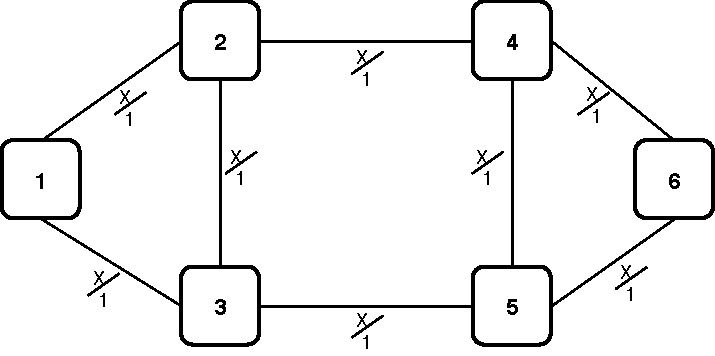
\includegraphics[width=13cm]{sdf/ilp/transparent_protection/figures/allowed_physical_topology}
\caption{Allowed Physical Topology. The allowed physical topology is defined by the duct and sites in the field. It is assumed that each duct supports up to 1 bidirectional transmission system and each site supports up to 1 node.}
\label{allowed2_physical_protectionlow}
\end{figure}

\begin{figure}[h!]
\centering
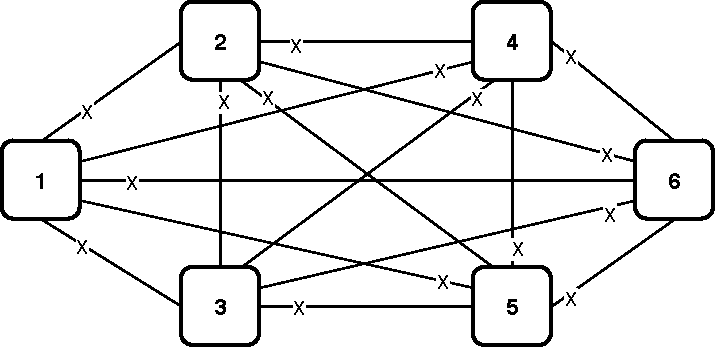
\includegraphics[width=13cm]{sdf/ilp/transparent_protection/figures/allowed_optical_topology}
\caption{Allowed Optical Topology. The allowed optical topology is defined by the transport mode (transparent transport mode in this case). It is assumed that each connections between demands supports up to 100 lightpaths.}
\label{allowed2_optical_protectionlow}
\end{figure}

\newpage
\begin{figure}[h!]
\centering
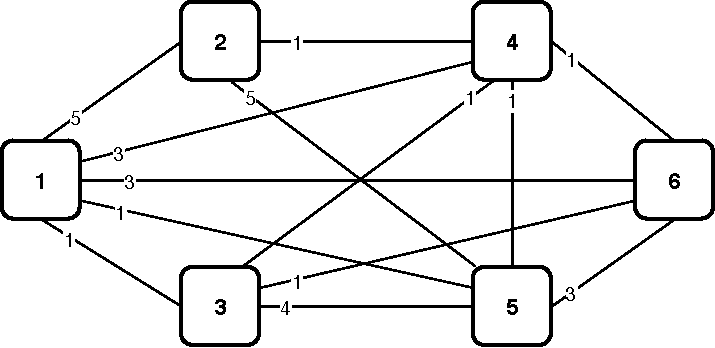
\includegraphics[width=12cm]{sdf/ilp/transparent_protection/figures/logical_topology_ODU0_low}
\caption{Logical Topology defined by the ODU0 traffic matrix.}
\label{logical2_ODU0_protectionlow}
\end{figure}

\begin{figure}[h!]
\centering
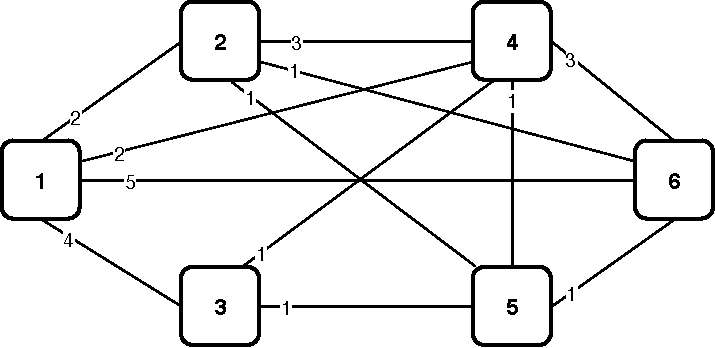
\includegraphics[width=12cm]{sdf/ilp/transparent_protection/figures/logical_topology_ODU1_low}
\caption{Logical Topology defined by the ODU1 traffic matrix.}
\label{logical2_ODU1_protectionlow}
\end{figure}

\begin{figure}[h!]
\centering
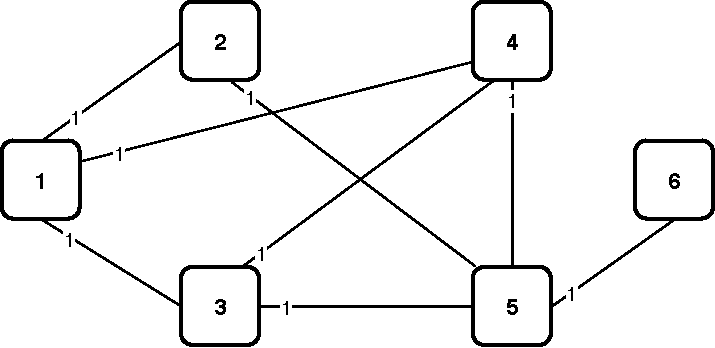
\includegraphics[width=12cm]{sdf/ilp/transparent_protection/figures/logical_topology_ODU2_low}
\caption{Logical Topology defined by the ODU2 traffic matrix.}
\label{logical2_ODU2_protectionlow}
\end{figure}

\begin{figure}[h!]
\centering
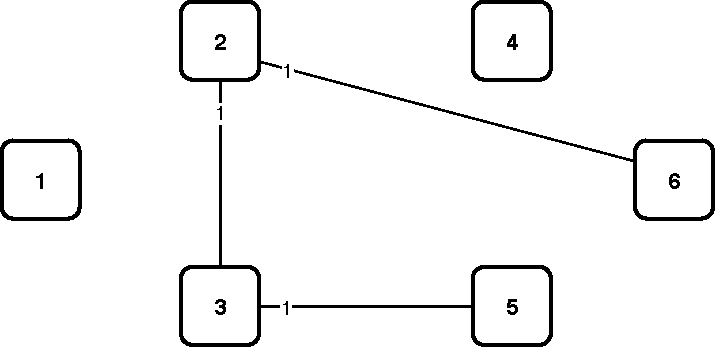
\includegraphics[width=12cm]{sdf/ilp/transparent_protection/figures/logical_topology_ODU3_low}
\caption{Logical Topology defined by the ODU3 traffic matrix.}
\label{logical2_ODU3_protectionlow}
\end{figure}

\begin{figure}[h!]
\centering
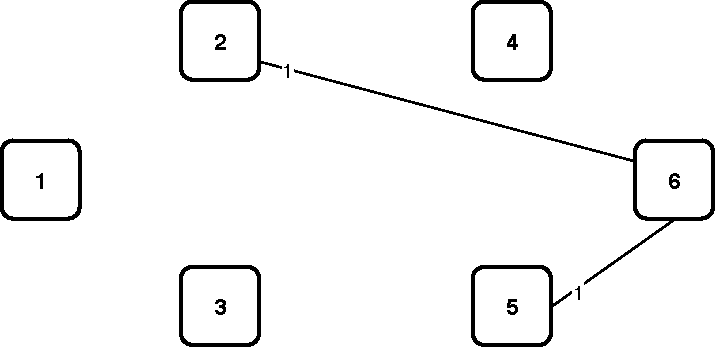
\includegraphics[width=12cm]{sdf/ilp/transparent_protection/figures/logical_topology_ODU4_low}
\caption{Logical Topology defined by the ODU4 traffic matrix.}
\label{logical2_ODU4_protectionlow}
\end{figure}

\begin{figure}[h!]
\centering
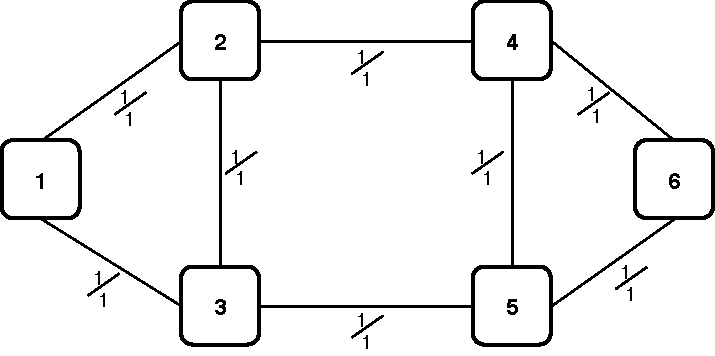
\includegraphics[width=12cm]{sdf/ilp/transparent_protection/figures/physical_topology}
\caption{Physical Topology after dimensioning.}
\label{physical2_protectionlow}
\end{figure}

\begin{figure}[h!]
\centering
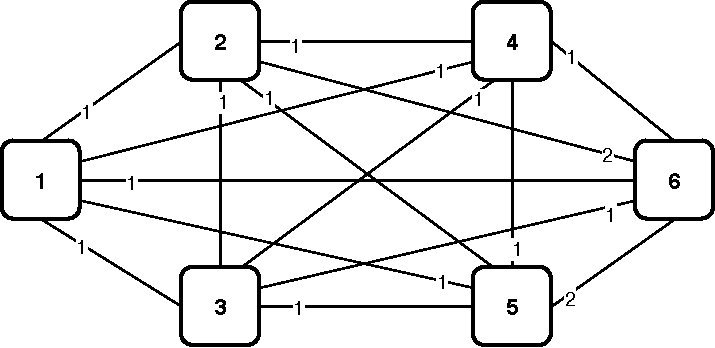
\includegraphics[width=12cm]{sdf/ilp/transparent_protection/figures/optical_topology_low}
\caption{Optical Topology after dimensioning.}
\label{optical2_protectionlow}
\end{figure}

In table \ref{link_transp_protec_ref_low} we can see the number of optical channels calculated using \ref{Capex_Link} and \ref{ILPOpaque_CAPEX} and the number of amplifiers for each link calculated using \ref{Capex_amplifiers}.

\begin{table}[h!]
\centering
\begin{tabular}{|| c | c | c ||}
 \hline
 \multicolumn{3}{|| c ||}{Information regarding links} \\
 \hline
 \hline
 Bidirectional Link & Optical Channels & Amplifiers\\
 \hline
 Node 1 <-> Node 2 & 6 & 4 \\
 Node 1 <-> Node 3 & 6 & 6 \\
 Node 2 <-> Node 3 & 10 & 0 \\
 Node 2 <-> Node 4 & 10 & 6 \\
 Node 3 <-> Node 5 & 10 & 8 \\
 Node 4 <-> Node 5 & 10 & 1 \\
 Node 4 <-> Node 6 & 8 & 7 \\
 Node 5 <-> Node 6 & 8 & 3 \\
 \hline
\end{tabular}
\caption{Table with information regarding links}
\label{link_transp_protec_ref_low}
\end{table}

In table \ref{node_transp_protec_ref_low} we can see the resulting nodal degree at the physical layer, the number of line ports the number of add ports and the number of tributary ports for each node.

\begin{table}[h!]
\centering
\begin{tabular}{|| c | c | c | c | c ||}
 \hline
 \multicolumn{5}{|| c ||}{Information regarding nodes} \\
 \hline
 \hline
 Node & Resulting Nodal Degree & Line Ports & Add Ports & Tributary Ports\\
 \hline
 1 & 2 & 12 & 5 & 29 \\
 2 & 3 & 26 & 6 & 23 \\
 3 & 3 & 26 & 5 & 18 \\
 4 & 3 & 28 & 5 & 20 \\
 5 & 3 & 28 & 6 & 24 \\
 6 & 2 & 16 & 7 & 22 \\
\hline
\end{tabular}
\caption{Table with information regarding nodes}
\label{node_transp_protec_ref_low}
\end{table}

\newpage
Through the information obtained previously on the nodes we can now create tables with detailed information about each node. In each table mentioned below we can see how many ports are connected to a given node and its bit rate (in relation to the line ports and the add ports) and how many ports are assigned to each different bit rate (in relation to the tributary ports).\\

\begin{table}[h!]
\centering
\begin{tabular}{|| c | c | c ||}
 \hline
 \multicolumn{3}{|| c ||}{Detailed description of Node 1} \\
 \hline
 \hline
  & Node<--Optical Channels-->Node & Bit rate \\
 \hline
 \multirow{2}{*}{12 line ports} & 1  <---- 6 ---->  2 & \multirow{7}{*}{100 Gbits/s} \\
  & 1  <---- 6 ---->  3 & \\ \cline{1-2}
 \multirow{5}{*}{5 add ports} & 1  <---- 1 ---->  2 & \\
  & 1  <---- 1 ---->  3 & \\
  & 1  <---- 1 ---->  4 & \\
  & 1  <---- 1 ---->  5 & \\
  & 1  <---- 1 ---->  6 & \\
 \hline
 \hline
  & Number of tributary ports & Bit rate \\ \hline
\multirow{3}{*}{29 tributary ports} & 13 & ODU0 \\
 & 13 & ODU1 \\
 & 3 & ODU2 \\
\hline
\end{tabular}
\caption{Table with detailed description of node 1}
\end{table}

\vspace{13pt}
\begin{table}[h!]
\centering
\begin{tabular}{|| c | c | c ||}
 \hline
 \multicolumn{3}{|| c ||}{Detailed description of Node 2} \\
 \hline
 \hline
  & Node<--Optical Channels-->Node & Bit rate \\
 \hline
 \multirow{3}{*}{26 line ports} & 2  <---- 6 ---->  1 & \multirow{8}{*}{100 Gbits/s} \\
  & 2  <---- 10 ---->  3 & \\
  & 2  <---- 10 ---->  4 & \\ \cline{1-2}
 \multirow{5}{*}{6 add ports} & 2  <---- 1 ---->  1 & \\
  & 2  <---- 1 ---->  3 & \\
  & 2  <---- 1 ---->  4 & \\
  & 2  <---- 1 ---->  5 & \\
  & 2  <---- 2 ---->  6 & \\
 \hline
 \hline
  & Number of tributary ports & Bit rate \\ \hline
\multirow{5}{*}{23 tributary ports} & 11 & ODU0 \\
 & 7 & ODU1 \\
 & 2 & ODU2 \\
 & 2 & ODU3 \\
 & 1 & ODU4 \\
\hline
\end{tabular}
\caption{Table with detailed description of node 2}
\end{table}

\newpage
\begin{table}[h!]
\centering
\begin{tabular}{|| c | c | c ||}
 \hline
 \multicolumn{3}{|| c ||}{Detailed description of Node 3} \\
 \hline
 \hline
  & Node<--Optical Channels-->Node & Bit rate \\
 \hline
 \multirow{3}{*}{26 line ports} & 3  <---- 6 ---->  1 & \multirow{8}{*}{100 Gbits/s} \\
  & 3  <---- 10 ---->  2 & \\
  & 3  <---- 10 ---->  3 & \\ \cline{1-2}
 \multirow{5}{*}{5 add ports} & 3  <---- 1 ---->  1 & \\
  & 3  <---- 1 ---->  2 & \\
  & 3  <---- 1 ---->  4 & \\
  & 3  <---- 1 ---->  5 & \\
  & 3  <---- 1 ---->  6 & \\
 \hline
 \hline
  & Number of tributary ports & Bit rate \\ \hline
\multirow{4}{*}{18 tributary ports} & 7 & ODU0 \\
 & 6 & ODU1\\
 & 3 & ODU2\\
 & 2 & ODU3\\
\hline
\end{tabular}
\caption{Table with detailed description of node 3}
\end{table}

\vspace{20pt}
\begin{table}[h!]
\centering
\begin{tabular}{|| c | c | c ||}
 \hline
 \multicolumn{3}{|| c ||}{Detailed description of Node 4} \\
 \hline
 \hline
  & Node<--Optical Channels-->Node & Bit rate \\
 \hline
 \multirow{3}{*}{28 line ports} & 4  <---- 10 ---->  2 & \multirow{8}{*}{100 Gbits/s} \\
  & 4  <---- 10 ---->  5 & \\
  & 4  <---- 8 ---->  6 & \\ \cline{1-2}
 \multirow{5}{*}{5 add ports} & 4  <---- 1 ---->  1 & \\
  & 4  <---- 1 ---->  2 & \\
  & 4  <---- 1 ---->  3 & \\
  & 4  <---- 1 ---->  5 & \\
  & 4  <---- 1 ---->  6 & \\
 \hline
 \hline
  & Number of tributary ports & Bit rate \\ \hline
\multirow{3}{*}{20 tributary ports} & 7 & ODU0 \\
 & 10 & ODU1 \\
 & 3 & ODU2 \\
\hline
\end{tabular}
\caption{Table with detailed description of node 4}
\end{table}

\newpage
\begin{table}[h!]
\centering
\begin{tabular}{|| c | c | c ||}
 \hline
 \multicolumn{3}{|| c ||}{Detailed description of Node 5} \\
 \hline
 \hline
  & Node<--Optical Channels-->Node & Bit rate \\
 \hline
 \multirow{3}{*}{28 line ports} & 5  <---- 10 ---->  3 & \multirow{8}{*}{100 Gbits/s} \\
  & 5  <---- 10 ---->  4 & \\
  & 5  <---- 8 ---->  6 & \\ \cline{1-2}
 \multirow{5}{*}{6 add ports} & 5  <---- 1 ---->  1 & \\
  & 5  <---- 1 ---->  2 & \\
  & 5  <---- 1 ---->  3 & \\
  & 5  <---- 1 ---->  4 & \\
  & 5  <---- 2 ---->  6 & \\
 \hline
 \hline
  & Number of tributary ports & Bit rate \\ \hline
\multirow{5}{*}{24 tributary ports} & 14 & ODU0 \\
 & 4 & ODU1 \\
 & 4 & ODU2 \\
 & 1 & ODU3 \\
 & 1 & ODU4 \\
\hline
\end{tabular}
\caption{Table with detailed description of node 5}
\end{table}

\vspace{20pt}
\begin{table}[h!]
\centering
\begin{tabular}{|| c | c | c ||}
 \hline
 \multicolumn{3}{|| c ||}{Detailed description of Node 6} \\
 \hline
 \hline
  & Node<--Optical Channels-->Node & Bit rate \\
 \hline
 \multirow{2}{*}{16 line ports} & 6  <---- 8 ---->  4 & \multirow{7}{*}{100 Gbits/s} \\
  & 6  <---- 8 ---->  5 & \\ \cline{1-2}
 \multirow{5}{*}{7 add ports} & 6  <---- 1 ---->  1 & \\
  & 6  <---- 2 ---->  2 & \\
  & 6  <---- 1 ---->  3 & \\
  & 6  <---- 1 ---->  4 & \\
  & 6  <---- 2 ---->  5 & \\
 \hline
 \hline
  & Number of tributary ports & Bit rate \\ \hline
\multirow{5}{*}{22 tributary ports} & 8 & ODU0 \\
 & 10 & ODU1 \\
 & 1 & ODU2 \\
 & 1 & ODU3 \\
 & 2 & ODU4 \\
\hline
\end{tabular}
\caption{Table with detailed description of node 6}
\end{table}

\newpage
Now through the table \ref{scripttransp_protec_ref_low} we can see the result of CAPEX obtained with this ILP model.

\begin{table}[h!]
\centering
\begin{tabular}{|| c | c | c | c | c | c | c ||}
 \hline
 \multicolumn{7}{|| c ||}{CAPEX of the Network} \\
 \hline
 \hline
 \multicolumn{3}{|| c |}{ } & Quantity & Unit Price & Cost & Total \\
 \hline
 \multirow{3}{*}{Link Cost} & \multicolumn{2}{ c |}{OLTs} & 16 & 15 000 \euro & 240 000 \euro & \multirow{3}{*}{68 520 000 \euro} \\ \cline{2-6}
 & \multicolumn{2}{ c |}{100 Gb/s Transceivers} & 136 & 5 000 \euro/Gb/s & 68 000 000 \euro & \\ \cline{2-6}
 & \multicolumn{2}{ c |}{Amplifiers} & 70 & 4 000 \euro & 280 000 \euro & \\
 \hline
 \multirow{10}{*}{Node Cost} & \multirow{7}{*}{Electrical} & EXCs & 6 & 10 000 \euro & 60 000 \euro & \multirow{10}{*}{14 547 590 \euro} \\ \cline{3-6}
 & & ODU0 Ports & 60 & 10 \euro/port & 600 \euro & \\ \cline{3-6}
 & & ODU1 Ports & 50 & 15 \euro/port & 750 \euro & \\ \cline{3-6}
 & & ODU2 Ports & 16 & 30 \euro/port & 480 \euro & \\ \cline{3-6}
 & & ODU3 Ports & 8 & 60 \euro/port & 360 \euro & \\ \cline{3-6}
 & & ODU4 Ports & 4 & 100 \euro/port & 400 \euro & \\ \cline{3-6}
 & & Line Ports & 136 & 1 000 \euro/Gb/s & 13 600 000 \euro & \\ \cline{2-6}
 & \multirow{3}{*}{Optical} & OXCs & 6 & 20 000 \euro & 120 000 \euro & \\ \cline{3-6}
 & & Line Ports & 272 & 2 500 \euro/port & 680 000 \euro & \\ \cline{3-6}
 & & Add Ports & 34 & 2 500 \euro/port & 85 000 \euro & \\
 \hline
 \multicolumn{6}{|| c |}{Total Network Cost} & 83 067 590 \euro \\
\hline
\end{tabular}
\caption{Table with detailed description of CAPEX}
\label{scripttransp_protec_ref_low}
\end{table}


\vspace{11pt}
Finally let's focus on the routing information. In table \ref{path_transp_protec_ref_low} we can see all the routing obtained for all nodes.

\begin{table}[h!]
\centering
\begin{tabular}{|| c | c | c ||}
 \hline
 \multicolumn{3}{|| c ||}{Routing} \\
 \hline
 \hline
 o & d & Links \\
 \hline
 \multirow{2}{*}{1} & \multirow{2}{*}{2} & \{(1,3),(3,2)\} \\
 & & \{(1,2)\} \\ \hline
 \multirow{2}{*}{1} & \multirow{2}{*}{3} & \{(1,2),(2,3)\} \\
 & & \{(1,3)\} \\ \hline
 \multirow{2}{*}{1} & \multirow{2}{*}{4} & \{(1,3),(3,5),(5,4)\} \\
 & & \{(1,2),(2,4)\} \\ \hline
 \multirow{2}{*}{1} & \multirow{2}{*}{5} & \{(1,2),(2,4),(4,5)\} \\
 & & \{(1,3),(3,5)\} \\ \hline
 \multirow{2}{*}{1} & \multirow{2}{*}{6} & \{(1,3),(3,5),(5,6)\} \\
 & & \{(1,2),(2,4),(4,6)\} \\ \hline
 \multirow{2}{*}{2} & \multirow{2}{*}{3} & \{(2,1),(1,3)\} \\
 & & \{(2,3)\} \\ \hline
 \multirow{2}{*}{2} & \multirow{2}{*}{4} & \{(2,3),(3,5),(5,4)\} \\
 & & \{(2,4)\} \\ \hline
 \multirow{2}{*}{2} & \multirow{2}{*}{5} & \{(2,4),(4,5)\} \\
 & & \{(2,3),(3,5)\} \\ \hline
 \multirow{2}{*}{2} & \multirow{2}{*}{6} & \{(2,3),(3,5),(5,6)\} \\
 & & \{(2,4),(4,6)\} \\ \hline
 \multirow{2}{*}{3} & \multirow{2}{*}{4} & \{(3,5),(5,4)\} \\
 & & \{(3,2),(2,4)\} \\ \hline
 \multirow{2}{*}{3} & \multirow{2}{*}{5} & \{(3,2),(2,4),(4,5)\} \\
 & & \{(3,5)\} \\ \hline
 \multirow{2}{*}{3} & \multirow{2}{*}{6} & \{(3,2),(2,4),(4,6)\} \\
 & & \{(3,5),(5,6)\} \\ \hline
 \multirow{2}{*}{4} & \multirow{2}{*}{5} & \{(4,6),(6,5)\} \\
 & & \{(4,5)\} \\ \hline
 \multirow{2}{*}{4} & \multirow{2}{*}{6} & \{(4,5),(5,6)\} \\
 & & \{(4,6)\} \\ \hline
 \multirow{2}{*}{5} & \multirow{2}{*}{6} & \{(5,4),(4,6)\} \\
 & & \{(5,6)\} \\
 \hline
\end{tabular}
\caption{Table with description of routing}
\label{path_transp_protec_ref_low}
\end{table}


\newpage
\textbf{Medium Traffic Scenario:}\\



\textbf{High Traffic Scenario:}\\
